\documentclass[10pt]{beamer}

\usetheme{Warsaw}

\usepackage{amsmath}
%\usepackage[style=apa]{biblatex}
\usepackage{multimedia}

\author{George G Vega\thanks{\url{mailto:gvegayon@caltech.edu}}}
\institute{Superintendencia de Pensiones}
\title{An\'alisis de Redes}
\date{27 de junio, 2014}

\begin{document}

\frame{\maketitle}

\begin{frame}
\frametitle{Contenidos}
\tableofcontents
\end{frame}

\begin{frame}
\begin{itemize}
\item Resilencia: Algunas ideas.
\item Medidas de centralidad: Grado, Cercan\'ia, Intermediaci\'on
\item Estructura: Homofilia (assortative mixing), Algoritmos de clusterizaci\'on
\item 
\end{itemize}
\end{frame}

\begin{frame}
\begin{figure}
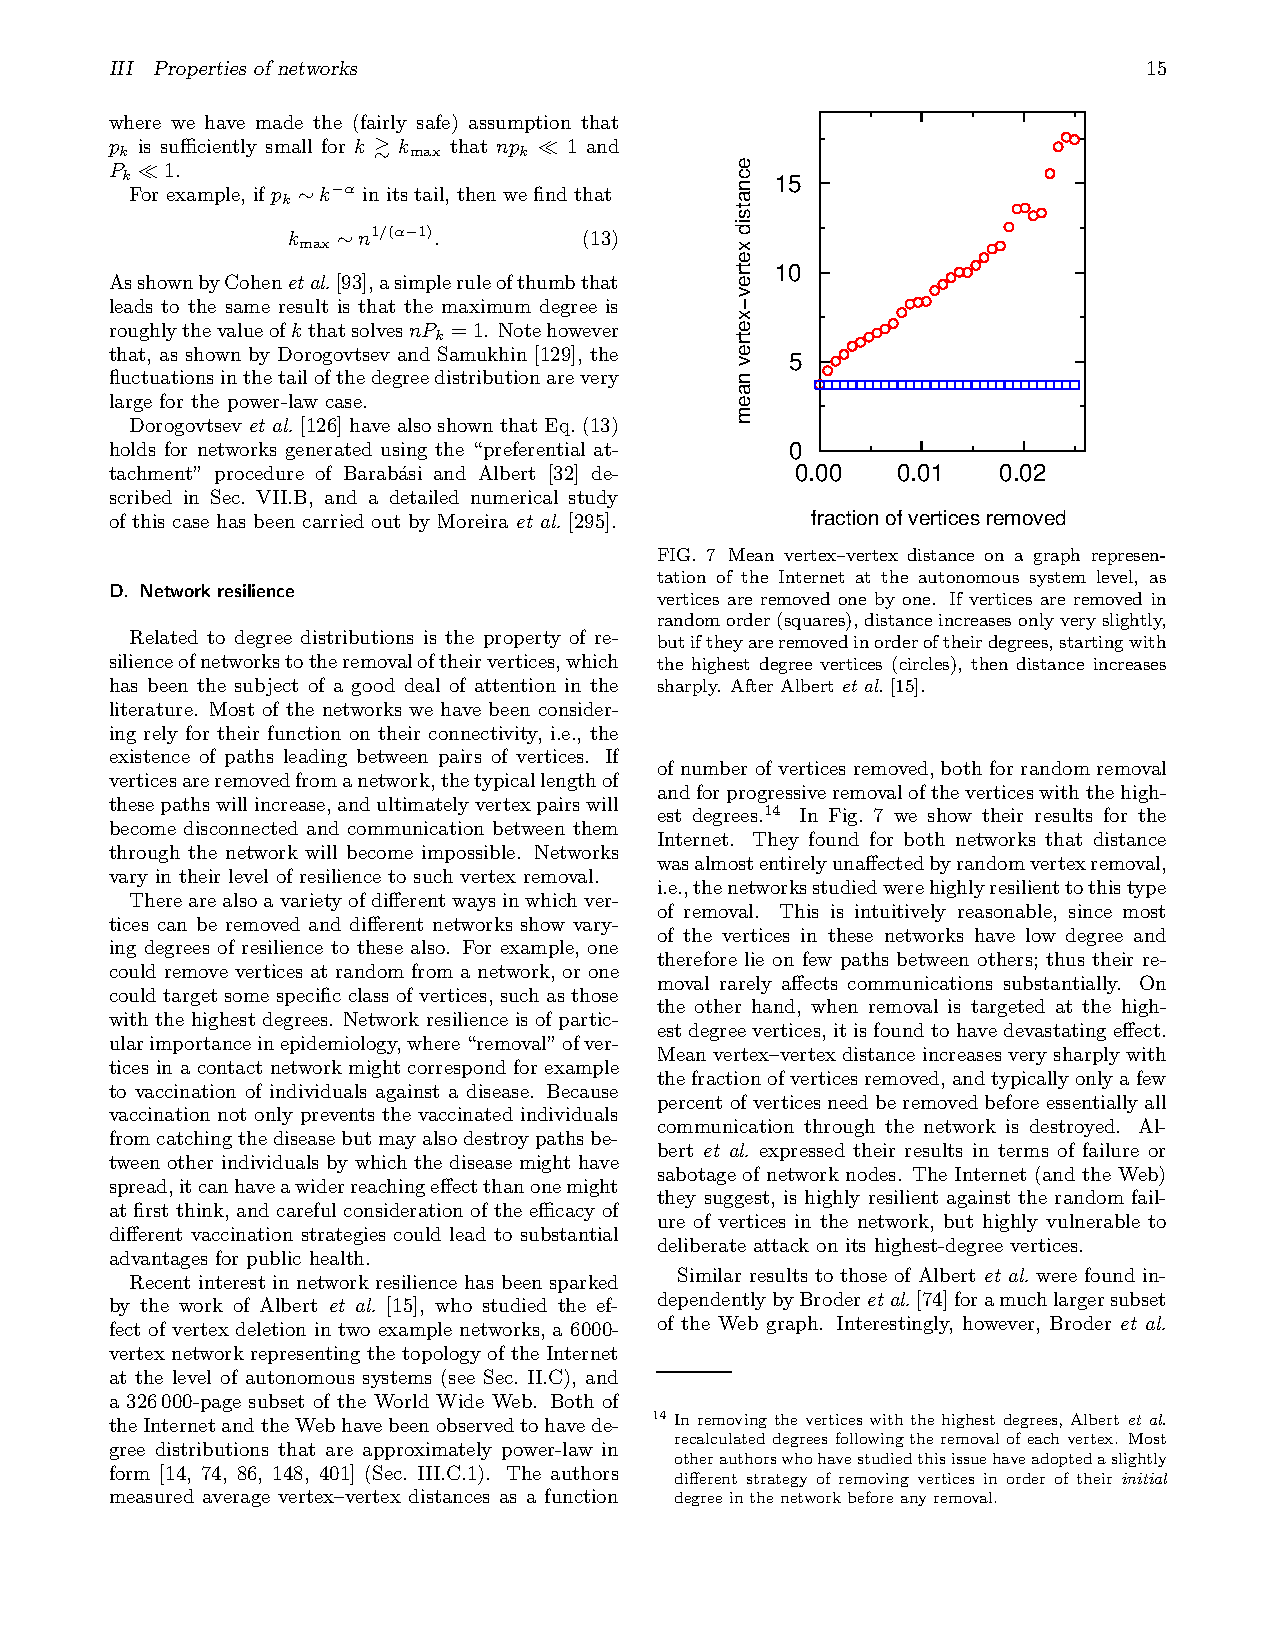
\includegraphics[trim=11cm 16cm 1.5cm 1.5cm, clip=true, width=.6\linewidth]{newman_network_resilense.pdf}
\end{figure}
{\footnotesize Fuente: Extraido del curso \emph{Social Network Analysis}, Lada
Adamic, University of Michigan \cite{lada2014}}
\end{frame}

\begin{frame}
\frametitle{Centralidad}
\framesubtitle{Comparaci\'on de tipos de centralidad}
\begin{figure}
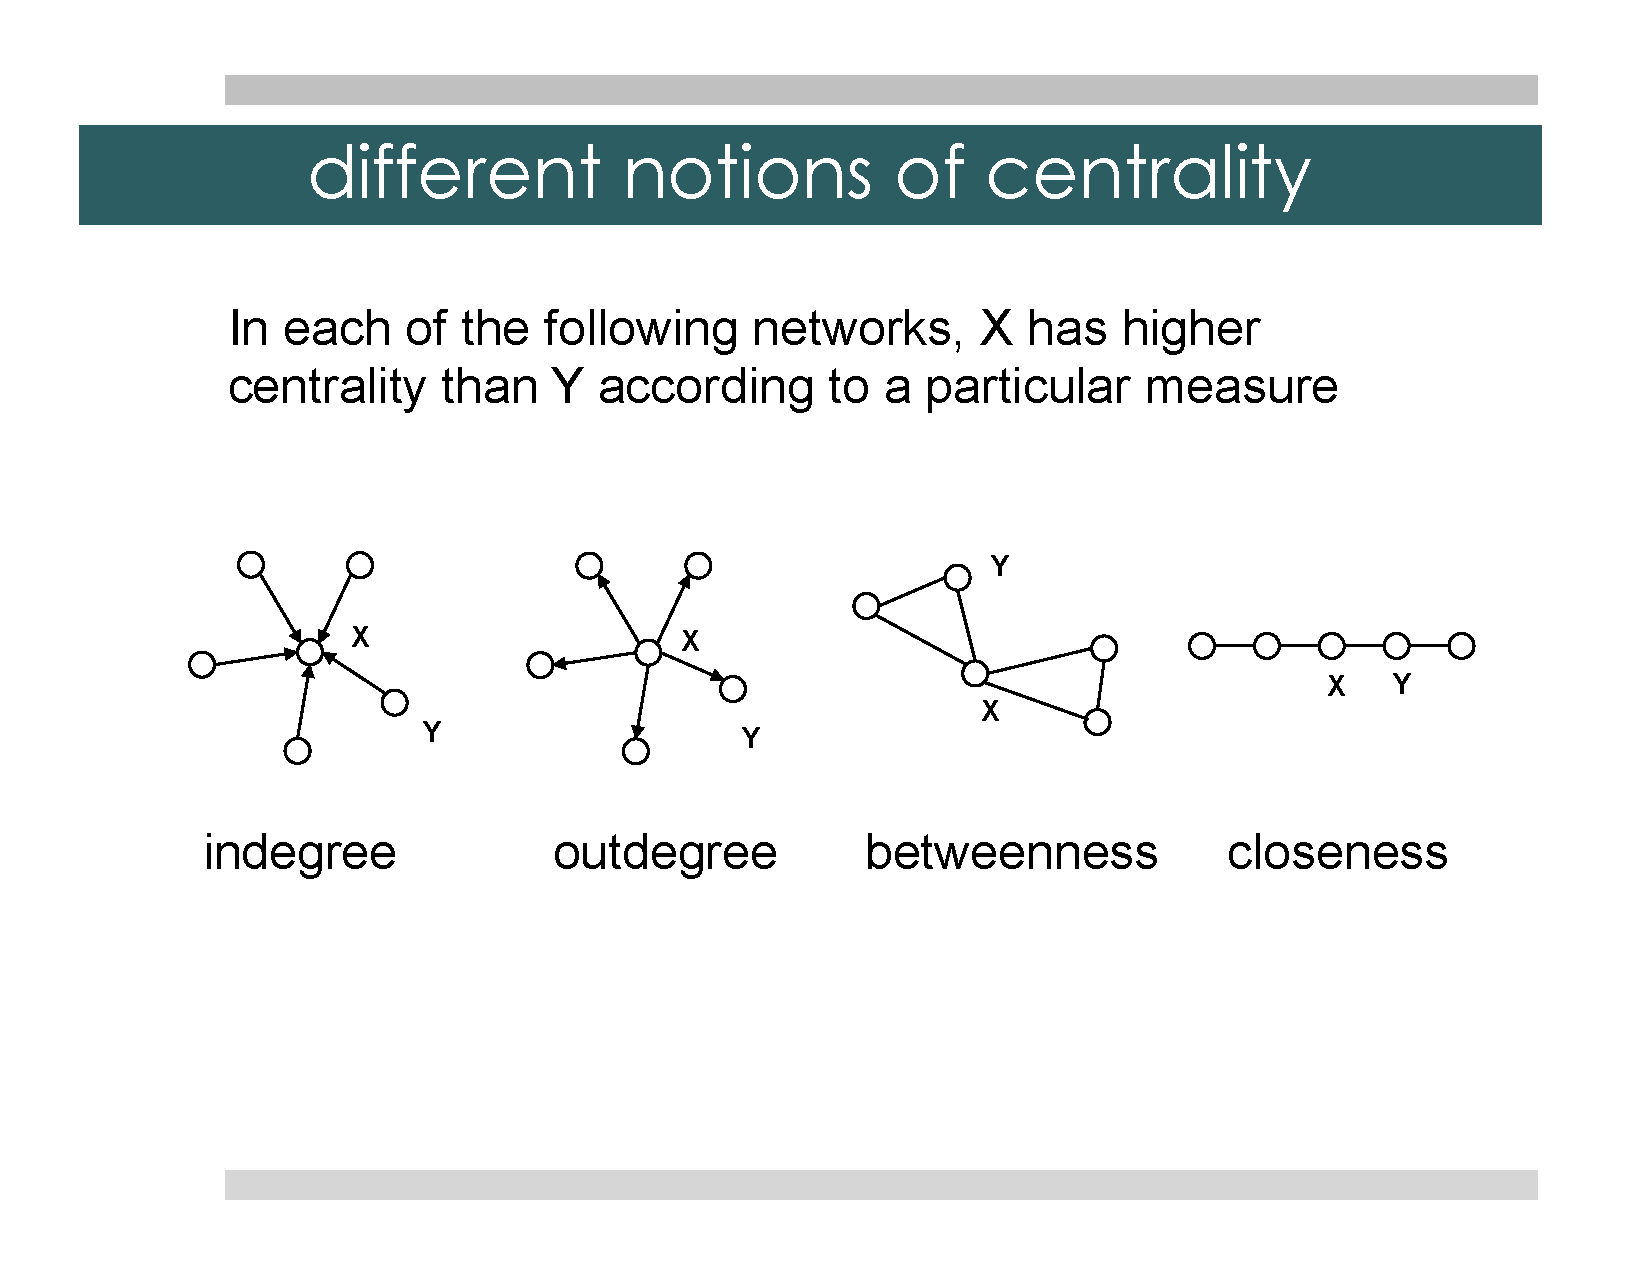
\includegraphics[trim=2cm 6cm 2cm 4cm, clip=true, width=\linewidth]{Lecture3Acentrality_comparison.pdf}
\end{figure}
{\footnotesize Fuente: Extraido de \emph{The structure and function of complex networks}, Newman (2003) \cite{newman2003structure}}
\end{frame}

\begin{frame}
\frametitle{Centralidad}
\framesubtitle{Intermediaci\'on (betweeness)}

\begin{quote}
[betweenness centrality] Se define como la porci\'on de veces que el nodo $i$ necesita al nojo $k$ (sobre
el cual se est\'a midiendo la centralidad) para alcanzar al nodo $j$.
Espec\'ificamente, si $g_{ij}$ es el n\'umero de rutas de $i$ a $j$, y $g_{ikj}$
es el n\'umero de geod\'esicas que pasa por el nodo $k$, entonces la centralidad
de intermediaci\'on est\'a dada por: 
\end{quote}

\begin{equation}
C_B=\sum_i\sum_j{\frac{g_{ikj}}{g_{ij}}}, i \neq j \neq k
\end{equation}

\begin{quote}
En t\'erminos sencillos, [...] b\'asicamente cuenta el n\'umero de geod\'esicas
que pasan a trav\'es del nodo $k$. \cite{borgatti2005centrality}
\end{quote}
\end{frame}

\begin{frame}
\frametitle{Centralidad}
\framesubtitle{PageRank}
\begin{figure}
\centering
\includegraphics[width=.8\linewidth]{PageRank-hi-res}
\end{figure}
{\footnotesize Caricatura de PageRank}
\end{frame}

\begin{frame}
\frametitle{Temas que revisaremos en la pr\'oxima sesi\'on}
\begin{itemize}
\item Centralidad de Grado (in/out)
\item Centralidad de Cercan\'ia
\item Centralidad de Intermediaci\'on
\end{itemize}
Otras medidas de centralidad...
\begin{itemize}
\item N\'umero de Erd{\"o}s 
\item El or\'aculo de Kevin Bacon \url{http://oracleofbacon.org/}
\end{itemize}
\end{frame}

\section{Referencias}
\begin{frame}
\frametitle{Referencias}
\bibliographystyle{plain}
\bibliography{../bib}
\end{frame}


\end{document}

